\documentclass[11pt]{article}
\usepackage[margin=1in]{geometry}
\usepackage[T1]{fontenc}
\usepackage{newtxtext,newtxmath}
\usepackage{graphicx}
\usepackage{booktabs}
\usepackage{tabularx}
\usepackage{array}
\usepackage{float}
\usepackage[section]{placeins}
\usepackage{caption}
\usepackage{amsmath}
\usepackage{enumitem}
\usepackage{tikz}
\usetikzlibrary{positioning,arrows.meta}
\usepackage[hidelinks]{hyperref}

\graphicspath{{figures/}}
\captionsetup{font=small,labelfont=bf}
\setlist{itemsep=2pt,topsep=4pt}
\newcolumntype{L}{>{\raggedright\arraybackslash}X}
\tikzset{box/.style={draw,rounded corners=3pt,fill=gray!10,align=center,font=\small,minimum height=0.8cm,inner sep=5pt},
         arr/.style={-{Stealth[length=2mm]}}}

\title{\textbf{Deep Learning-Based Vehicle Damage Localization and\\ Severity Assessment Using YOLO and CNNs}\\[6pt]
\large ENSE 812 Course Project Progress Report}
\author{\textbf{Md Rabiul Hasan}\\
Master of Engineering in Software Systems Engineering\\
University of Regina\\
ENSE 812 -- Applied Deep Learning with Computer Vision}
\date{October 29, 2026}

\begin{document}
\maketitle

\section{Introduction and Status Overview}

The approved proposal asked whether localizing vehicle damage with a YOLO detector before severity classification improves minor, moderate and severe classification compared with whole-image classification. It also asked whether localization helps the moderate class in particular. The proposal stated that a negative or mixed result would be meaningful if it came from a controlled experiment.

The project is on track. Ten of the eleven steps in the proposed workflow are complete or in progress, and both research questions have a first, controlled answer:

\begin{itemize}
  \item \textbf{Primary question.} With the current detector, localization did \emph{not} improve severity classification. On the held-out test set, the localized classifier reached a macro-F1 of 0.514 against 0.583 for the whole-image baseline.
  \item \textbf{Secondary question.} Moderate-class recall also fell, from 0.426 to 0.326.
  \item \textbf{Main cause.} The detector is a preliminary model. It finds nothing in about half of the severity images and often crops the wrong region, so detector errors propagate into the classifier. Section~10 of the proposal anticipated this outcome.
\end{itemize}

Using the measures defined in the proposal,
\begin{align}
\Delta F1 &= F1_{\text{localized}} - F1_{\text{whole-image}} = 0.514 - 0.583 = -0.069, \\
\Delta R_{\text{moderate}} &= R_{\text{localized, moderate}} - R_{\text{whole-image, moderate}} = 0.326 - 0.426 = -0.100.
\end{align}
The 95\% paired bootstrap interval for $\Delta F1$ is $[-0.121, -0.016]$, so the difference is unlikely to be chance. The remaining work tests whether a stronger detector and crops with more context change this answer.

\section{Progress Against the Proposed Workflow}

Table~\ref{tab:status} maps each step of the proposed workflow (proposal, Figure~4) to its current status.

\begin{table}[!htbp]
\centering
\caption{Status of the proposed workflow steps.}
\label{tab:status}
\small
\begin{tabularx}{\textwidth}{@{}l l L@{}}
\toprule
Proposal step & Status & What exists now \\
\midrule
Literature review & Not started & Proposal references only; write-up planned \\
Dataset selection & Done & CarDD for detection; Car Damage Severity Dataset for severity \\
Data preparation and annotation & Done & CarDD converted to YOLO format; severity data audited for leakage \\
Train whole-image baseline & Done & ResNet50, three seeds \\
Train YOLO damage detector & In progress & Preliminary YOLO11n, 10 epochs \\
Evaluate damage detection & In progress & Validation metrics and error analysis; CarDD test split unused \\
Extract detected damage regions & Done & Padded union crop with whole-image fallback \\
Train / evaluate localized classifier & Done & ResNet50 on crops, three seeds \\
Baseline vs.\ localized comparison & Done (round 1) & Validation and one test evaluation \\
Moderate-class and error analysis & In progress & Per-class recall, confusion matrices, error panels \\
Final implementation and demo & In progress & Local dashboard runs detection and severity \\
\bottomrule
\end{tabularx}
\end{table}

\section{Datasets and Data Preparation}

As the proposal allowed, detection and severity classification use separate datasets.

\paragraph{Detection: CarDD.} CarDD~\cite{cardd} provides 4,000 images with bounding boxes for six damage types. The COCO annotations were converted to YOLO format, and the six types were merged into a single ``damage'' class, because the severity stage needs the damage location, not its type. The original split gives 2,816 training, 810 validation and 374 test images. The test split has not been used yet.

\paragraph{Severity: Car Damage Severity Dataset.} This is the dataset used in the earlier projects, labelled minor, moderate and severe in a fixed training, validation and test split. Its images are small (median $259 \times 184$ pixels). Before any training, every image was checked for byte-identical and near-identical copies using a perceptual hash, and every flagged pair was confirmed visually (Figure~\ref{fig:audit}). Table~\ref{tab:audit} lists what was removed. Forty-two images were found to be copies of CarDD photos, which the detector was trained on; the copies in the validation and test splits were removed so that the detector is never evaluated on images it has seen.

\begin{table}[!htbp]
\centering
\caption{Images removed from the severity dataset by the leakage audit.}
\label{tab:audit}
\small
\begin{tabularx}{\textwidth}{@{}L r L@{}}
\toprule
Issue & Removed & Rule \\
\midrule
Duplicates within a split & 16 & Keep one copy \\
Duplicates across splits & 9 & Keep the training copy \\
Same image with conflicting labels & 4 & Remove all copies \\
Validation or test images also in CarDD & 27 & Remove; the detector was trained on CarDD \\
\bottomrule
\end{tabularx}
\end{table}

\begin{table}[!htbp]
\centering
\caption{Severity images used after filtering.}
\label{tab:split}
\small
\begin{tabular}{@{}lrrrr@{}}
\toprule
Split & Minor & Moderate & Severe & Total \\
\midrule
Training & 355 & 363 & 341 & 1,059 \\
Validation & 75 & 75 & 89 & 239 \\
Test & 67 & 86 & 92 & 245 \\
\bottomrule
\end{tabular}
\end{table}

\begin{figure}[!htbp]
\centering
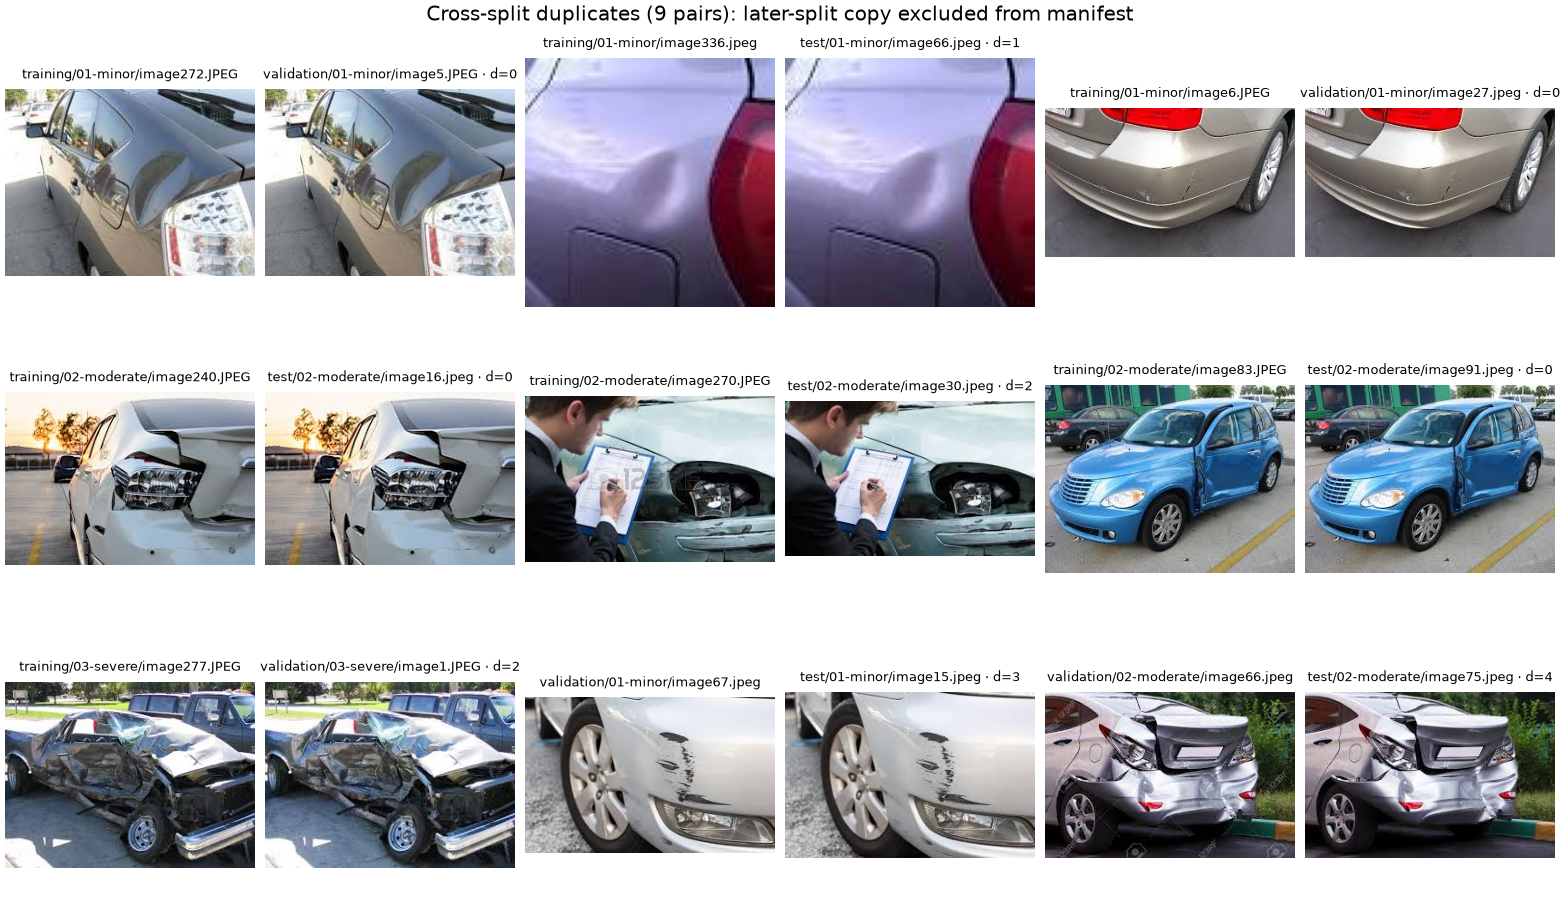
\includegraphics[width=\textwidth]{audit_cross_split.png}
\caption{Image pairs found in more than one split of the severity dataset. The later-split copy of each pair was removed.}
\label{fig:audit}
\end{figure}

\section{Damage Detection}

\paragraph{Setup.} A YOLO11n detector~\cite{yolo11} was trained on CarDD for 10 epochs at an image size of 640 with a batch size of 8 on an Apple MPS GPU. Before analysis, a controlled re-validation reproduced the saved metrics (Table~\ref{tab:det}).

\begin{table}[!htbp]
\centering
\caption{Detector validation metrics on 810 CarDD images: saved at epoch 10 and reproduced without retraining.}
\label{tab:det}
\small
\begin{tabular}{@{}lrr@{}}
\toprule
Metric & Saved & Reproduced \\
\midrule
Precision & 0.606 & 0.610 \\
Recall & 0.444 & 0.442 \\
mAP50 & 0.503 & 0.502 \\
mAP50--95 & 0.313 & 0.313 \\
\bottomrule
\end{tabular}
\end{table}

Validation mAP was still rising when training stopped (Figure~\ref{fig:dettrain}), so the detector is under-trained.

\begin{figure}[!htbp]
\centering
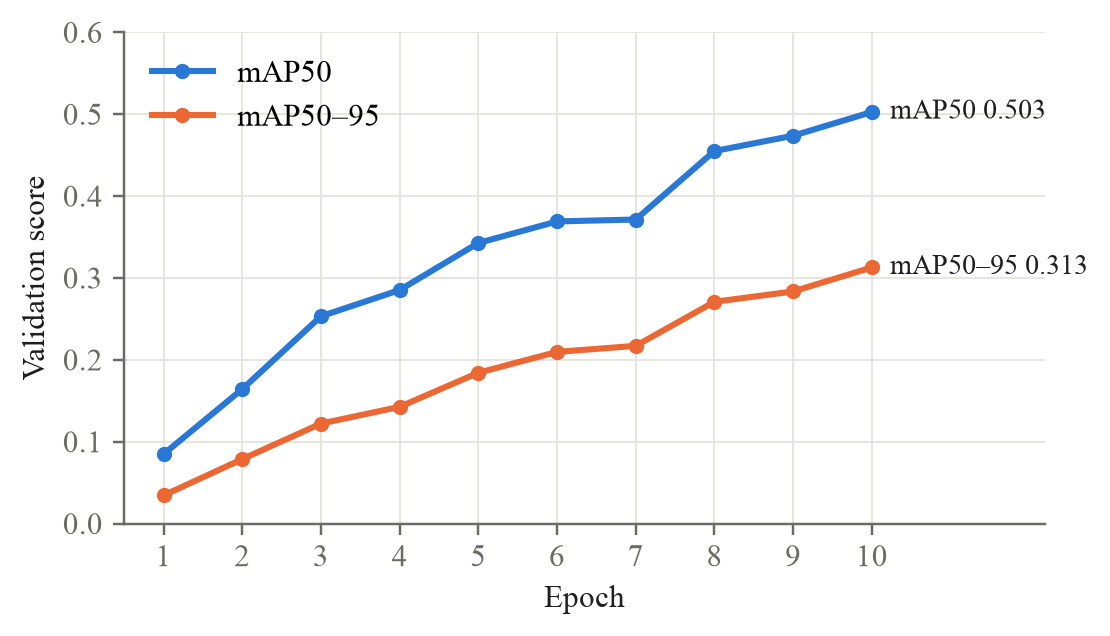
\includegraphics[width=0.78\textwidth]{detector_training.png}
\caption{Detector validation mAP by epoch, from the saved training log.}
\label{fig:dettrain}
\end{figure}

\paragraph{Confidence threshold.} The saved confusion matrix showed about 121,000 unmatched detections. An audit showed that this comes from the plotting threshold of 0.001, not from a model fault (Table~\ref{tab:thr}, Figure~\ref{fig:thr}). The operating threshold for cropping was fixed at 0.25 in advance.

\begin{table}[!htbp]
\centering
\caption{Detection counts at fixed confidence thresholds (matching IoU $>$ 0.45, 810 validation images).}
\label{tab:thr}
\small
\begin{tabular}{@{}rrrrr@{}}
\toprule
Confidence $>$ & False positives & Precision & Recall & Images with no detection \\
\midrule
0.001 & 120,956 & 1.4\% & 96.1\% & 0 \\
0.10 & 1,736 & 37.8\% & 60.4\% & 3 \\
0.25 & 391 & 66.3\% & 44.0\% & 88 \\
0.50 & 74 & 85.7\% & 25.5\% & 338 \\
\bottomrule
\end{tabular}
\end{table}

\begin{figure}[!htbp]
\centering
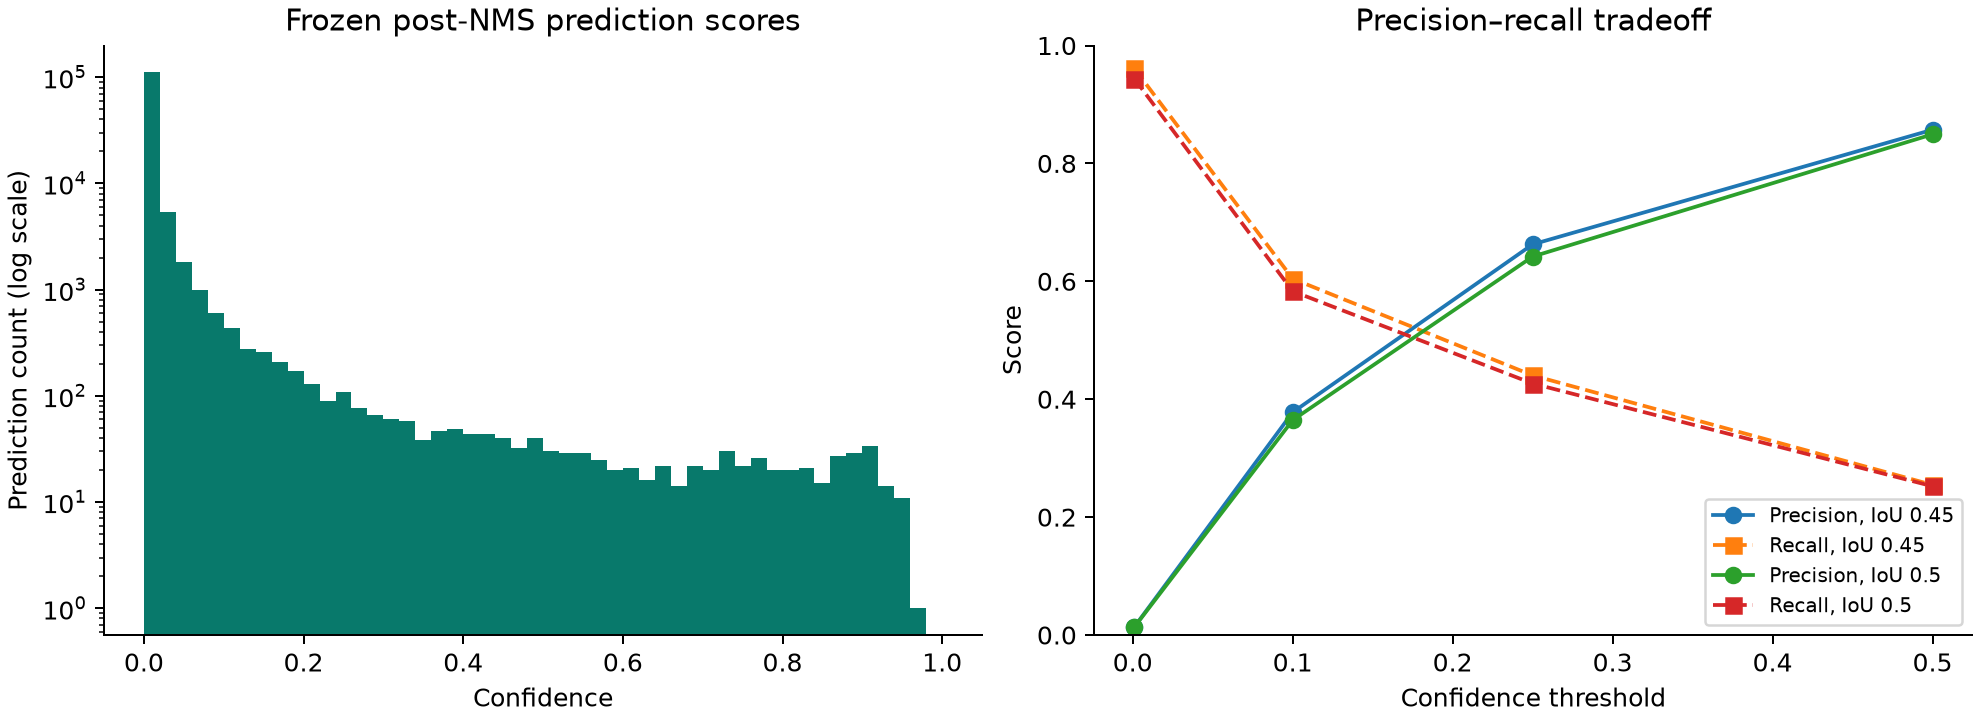
\includegraphics[width=\textwidth]{threshold_audit.png}
\caption{Left: distribution of prediction confidences. Right: precision and recall at fixed confidence thresholds.}
\label{fig:thr}
\end{figure}

\paragraph{Multiple damages.} Recall falls sharply as an image contains more damaged areas (Figure~\ref{fig:multi}). Even in images with five or more annotated areas, the detector predicts about two boxes on average. Visual inspection shows oversized boxes that cover several damages and missed regions next to an obvious one (Figure~\ref{fig:missed}).

\begin{figure}[!htbp]
\centering
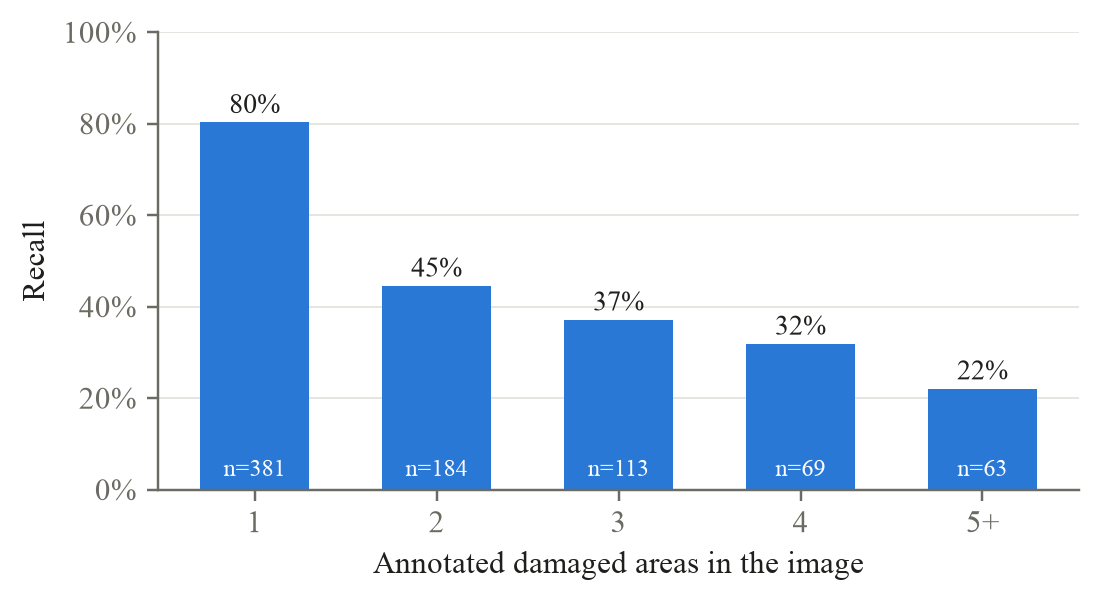
\includegraphics[width=0.78\textwidth]{recall_by_damage_count.png}
\caption{Detector recall by the number of annotated damaged areas per validation image (confidence $>$ 0.25, IoU $>$ 0.45).}
\label{fig:multi}
\end{figure}

\begin{figure}[!htbp]
\centering
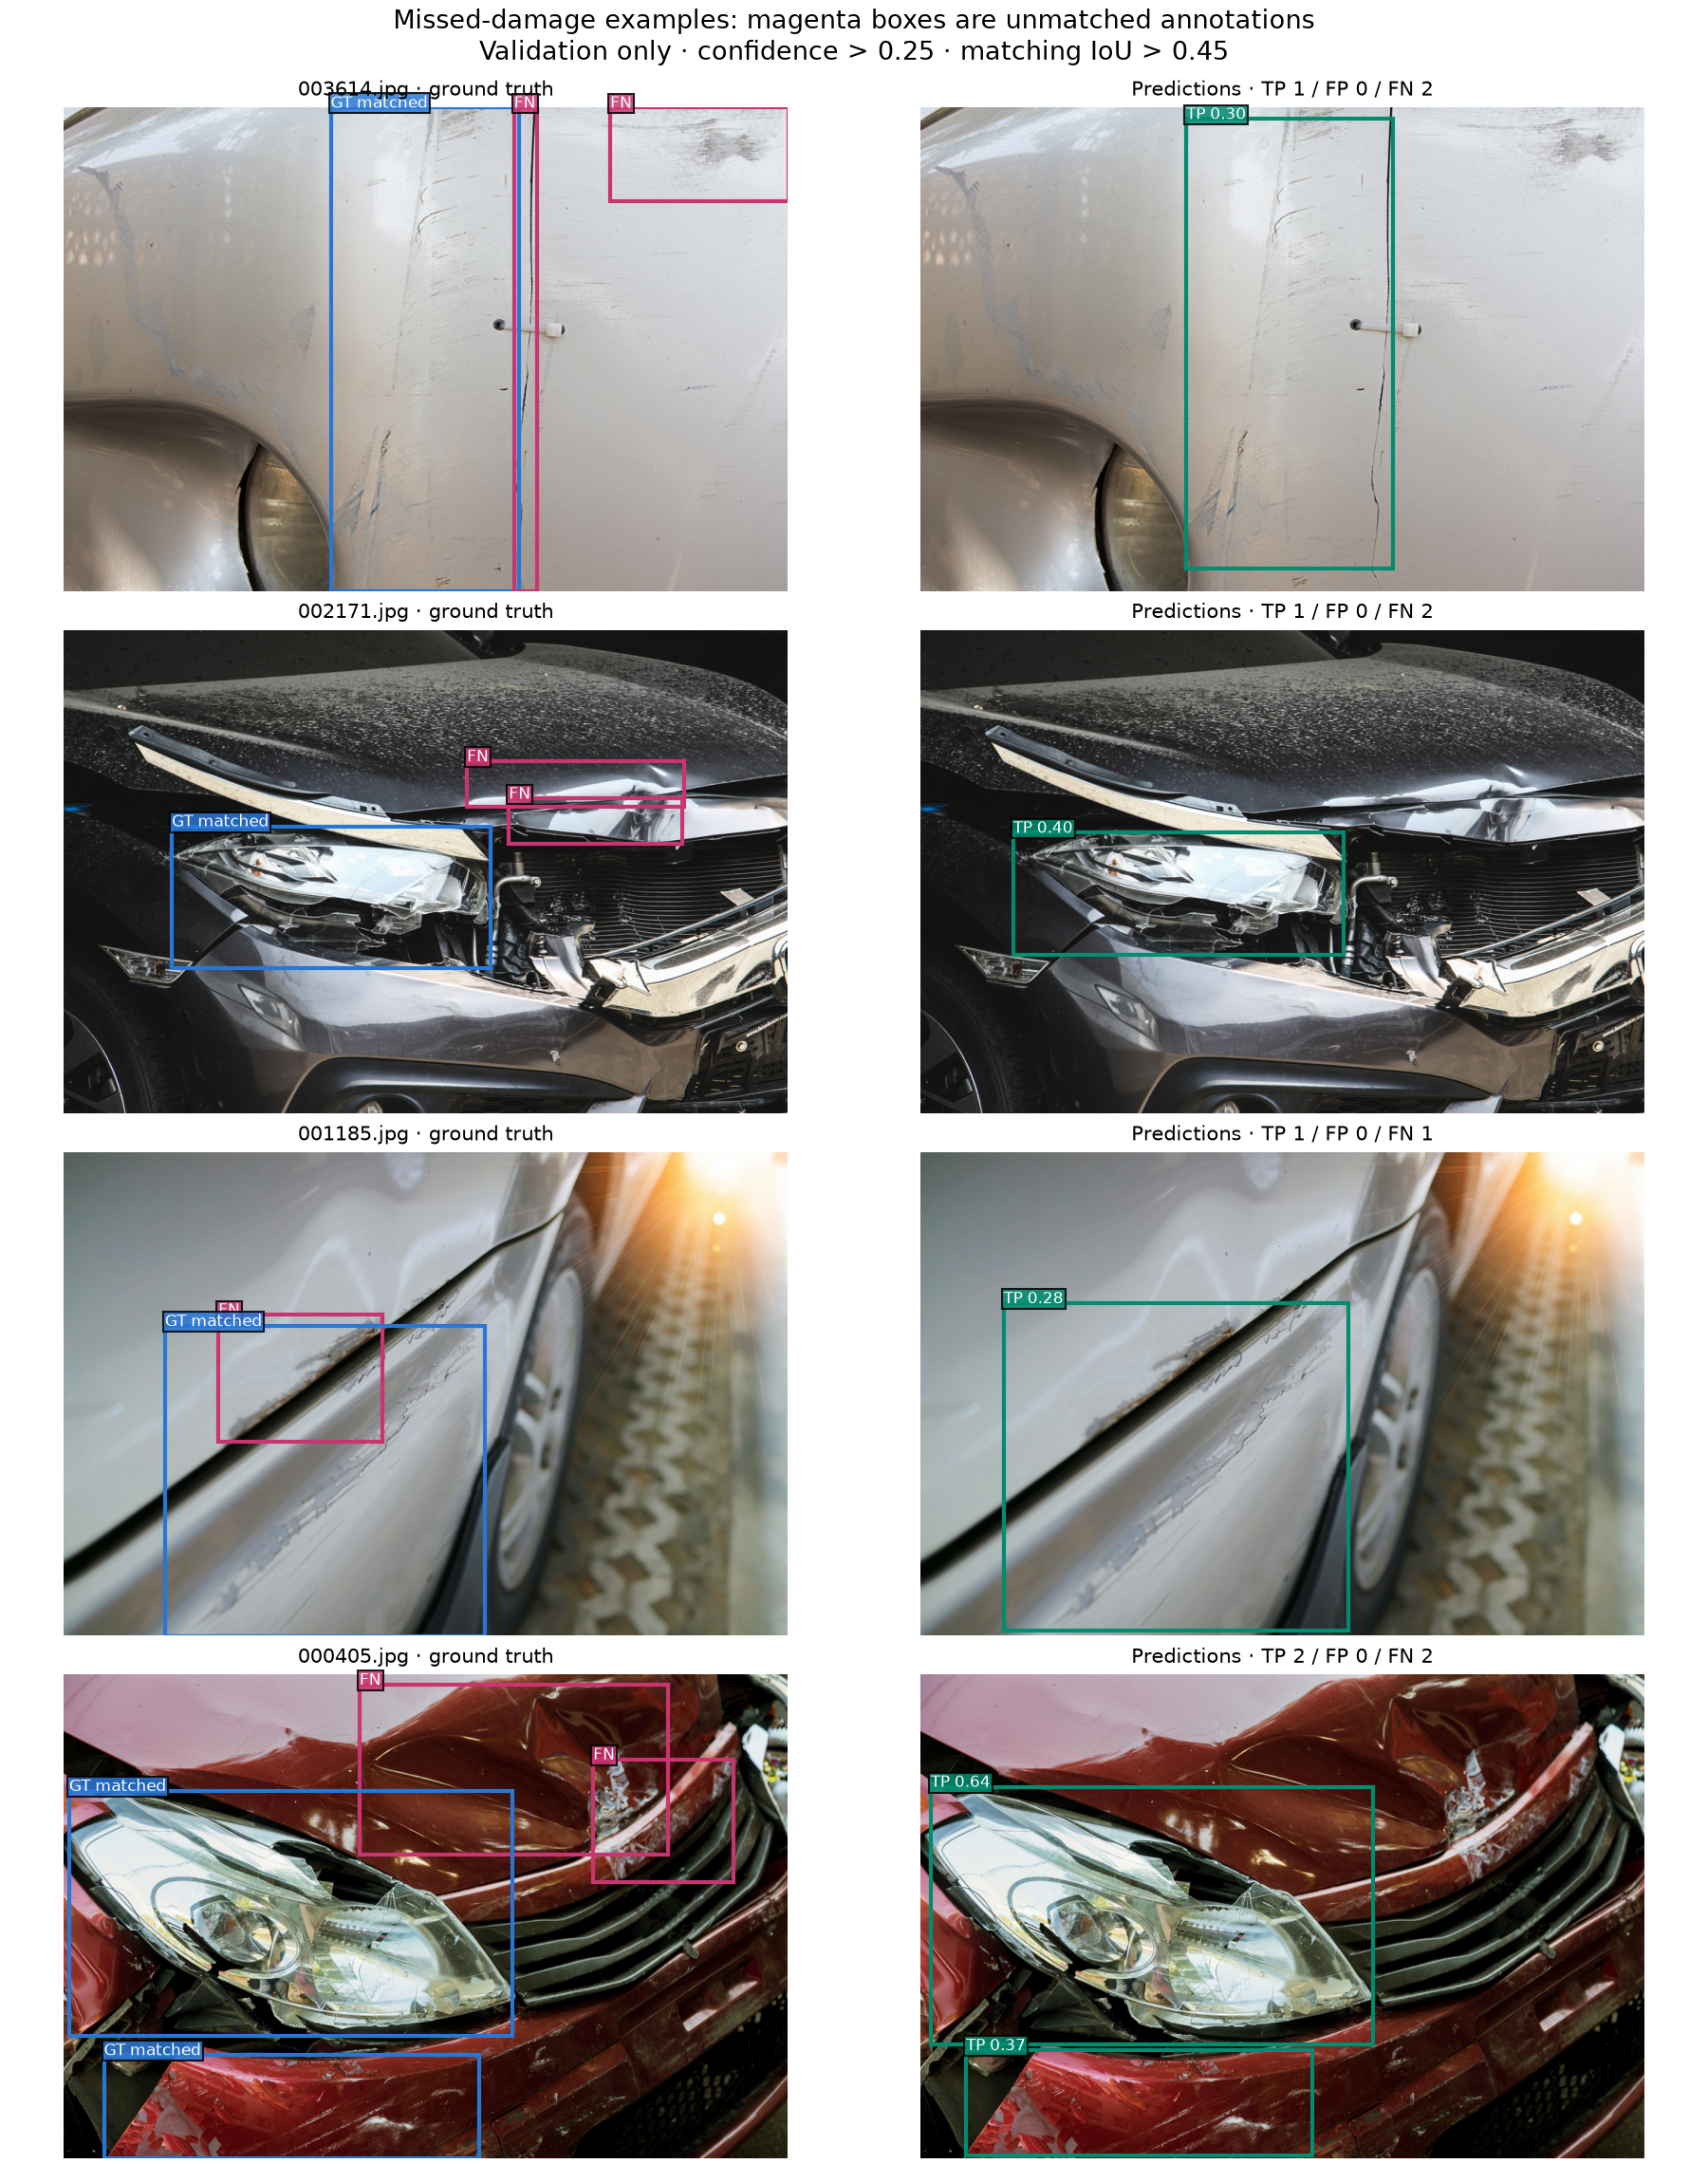
\includegraphics[width=0.92\textwidth]{detector_missed_damage.png}
\caption{Validation images with missed damage. Left: ground truth (blue matched, magenta missed). Right: predictions (green matched, orange unmatched).}
\label{fig:missed}
\end{figure}

\section{Severity Classification: Whole-Image vs.\ Localized}

\subsection{Experimental Design}

The two systems from the proposal were built with the same classifier and training recipe (Figure~\ref{fig:pipe}). All settings were fixed before training.

\begin{figure}[!htbp]
\centering
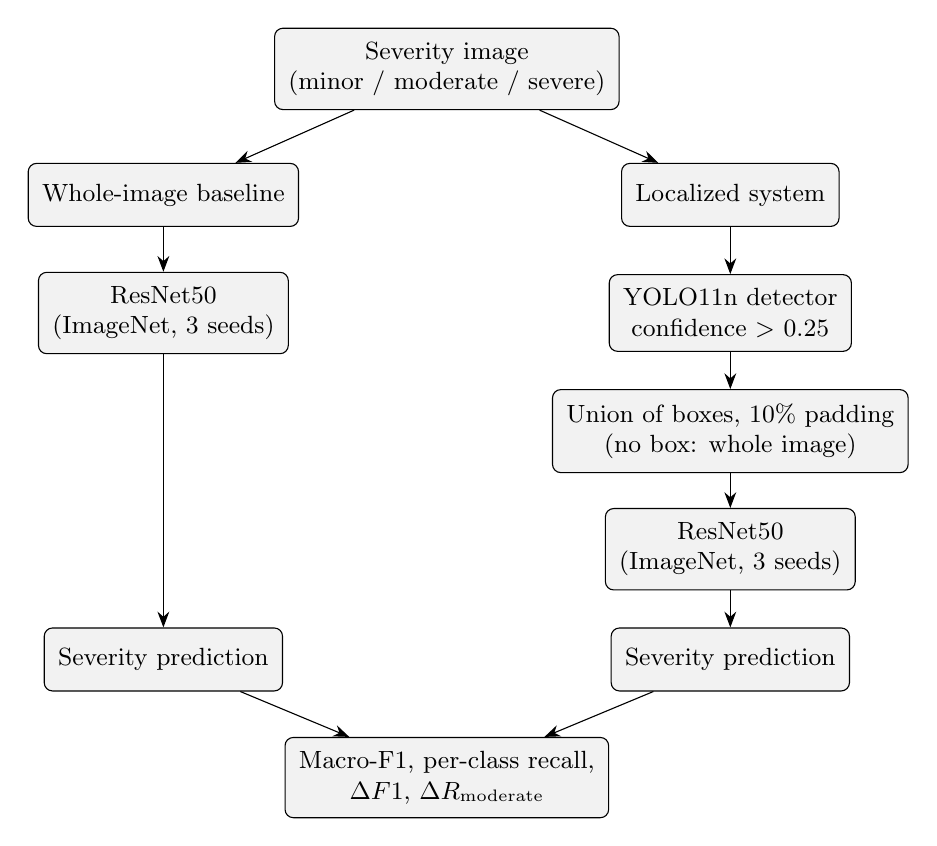
\begin{tikzpicture}
\node[box] (img) at (0,0) {Severity image\\(minor / moderate / severe)};
\node[box] (wb) at (-3.6,-1.6) {Whole-image baseline};
\node[box] (lb) at (3.6,-1.6) {Localized system};
\node[box] (wr) at (-3.6,-3.1) {ResNet50\\(ImageNet, 3 seeds)};
\node[box] (yolo) at (3.6,-3.1) {YOLO11n detector\\confidence $>$ 0.25};
\node[box] (crop) at (3.6,-4.6) {Union of boxes, 10\% padding\\(no box: whole image)};
\node[box] (lr) at (3.6,-6.1) {ResNet50\\(ImageNet, 3 seeds)};
\node[box] (wp) at (-3.6,-7.5) {Severity prediction};
\node[box] (lp) at (3.6,-7.5) {Severity prediction};
\node[box] (cmp) at (0,-9.0) {Macro-F1, per-class recall,\\$\Delta F1$, $\Delta R_{\text{moderate}}$};
\draw[arr] (img) -- (wb); \draw[arr] (img) -- (lb);
\draw[arr] (wb) -- (wr); \draw[arr] (wr) -- (wp);
\draw[arr] (lb) -- (yolo); \draw[arr] (yolo) -- (crop); \draw[arr] (crop) -- (lr); \draw[arr] (lr) -- (lp);
\draw[arr] (wp) -- (cmp); \draw[arr] (lp) -- (cmp);
\end{tikzpicture}
\caption{The comparison as implemented. Both branches use the same images, classifier, training recipe and seeds.}
\label{fig:pipe}
\end{figure}

\begin{itemize}
  \item \textbf{Damage region.} The union of all detections above confidence 0.25, padded by 10\% on each side. When nothing is detected, the whole image is used. This fallback applied to 49\% of training, 50\% of validation and 38\% of test images; these images were kept so that the test set is not biased toward easy cases.
  \item \textbf{Classifier.} ResNet50~\cite{resnet} with ImageNet weights and a new three-class head. Five epochs train only the head, then up to 25 epochs fine-tune all layers (AdamW, cosine schedule, label smoothing 0.1) with early stopping on validation macro-F1. Each system was trained with three seeds.
  \item \textbf{Test protocol.} The test split was evaluated once, after both systems and all checkpoints were fixed. Intervals are paired percentile bootstrap intervals over test images (2,000 resamples).
\end{itemize}

Figure~\ref{fig:crops} shows typical crops. Many land on a wheel, headlight or panel corner rather than the main damage, and heavily damaged cars are often not detected at all.

\begin{figure}[!htbp]
\centering
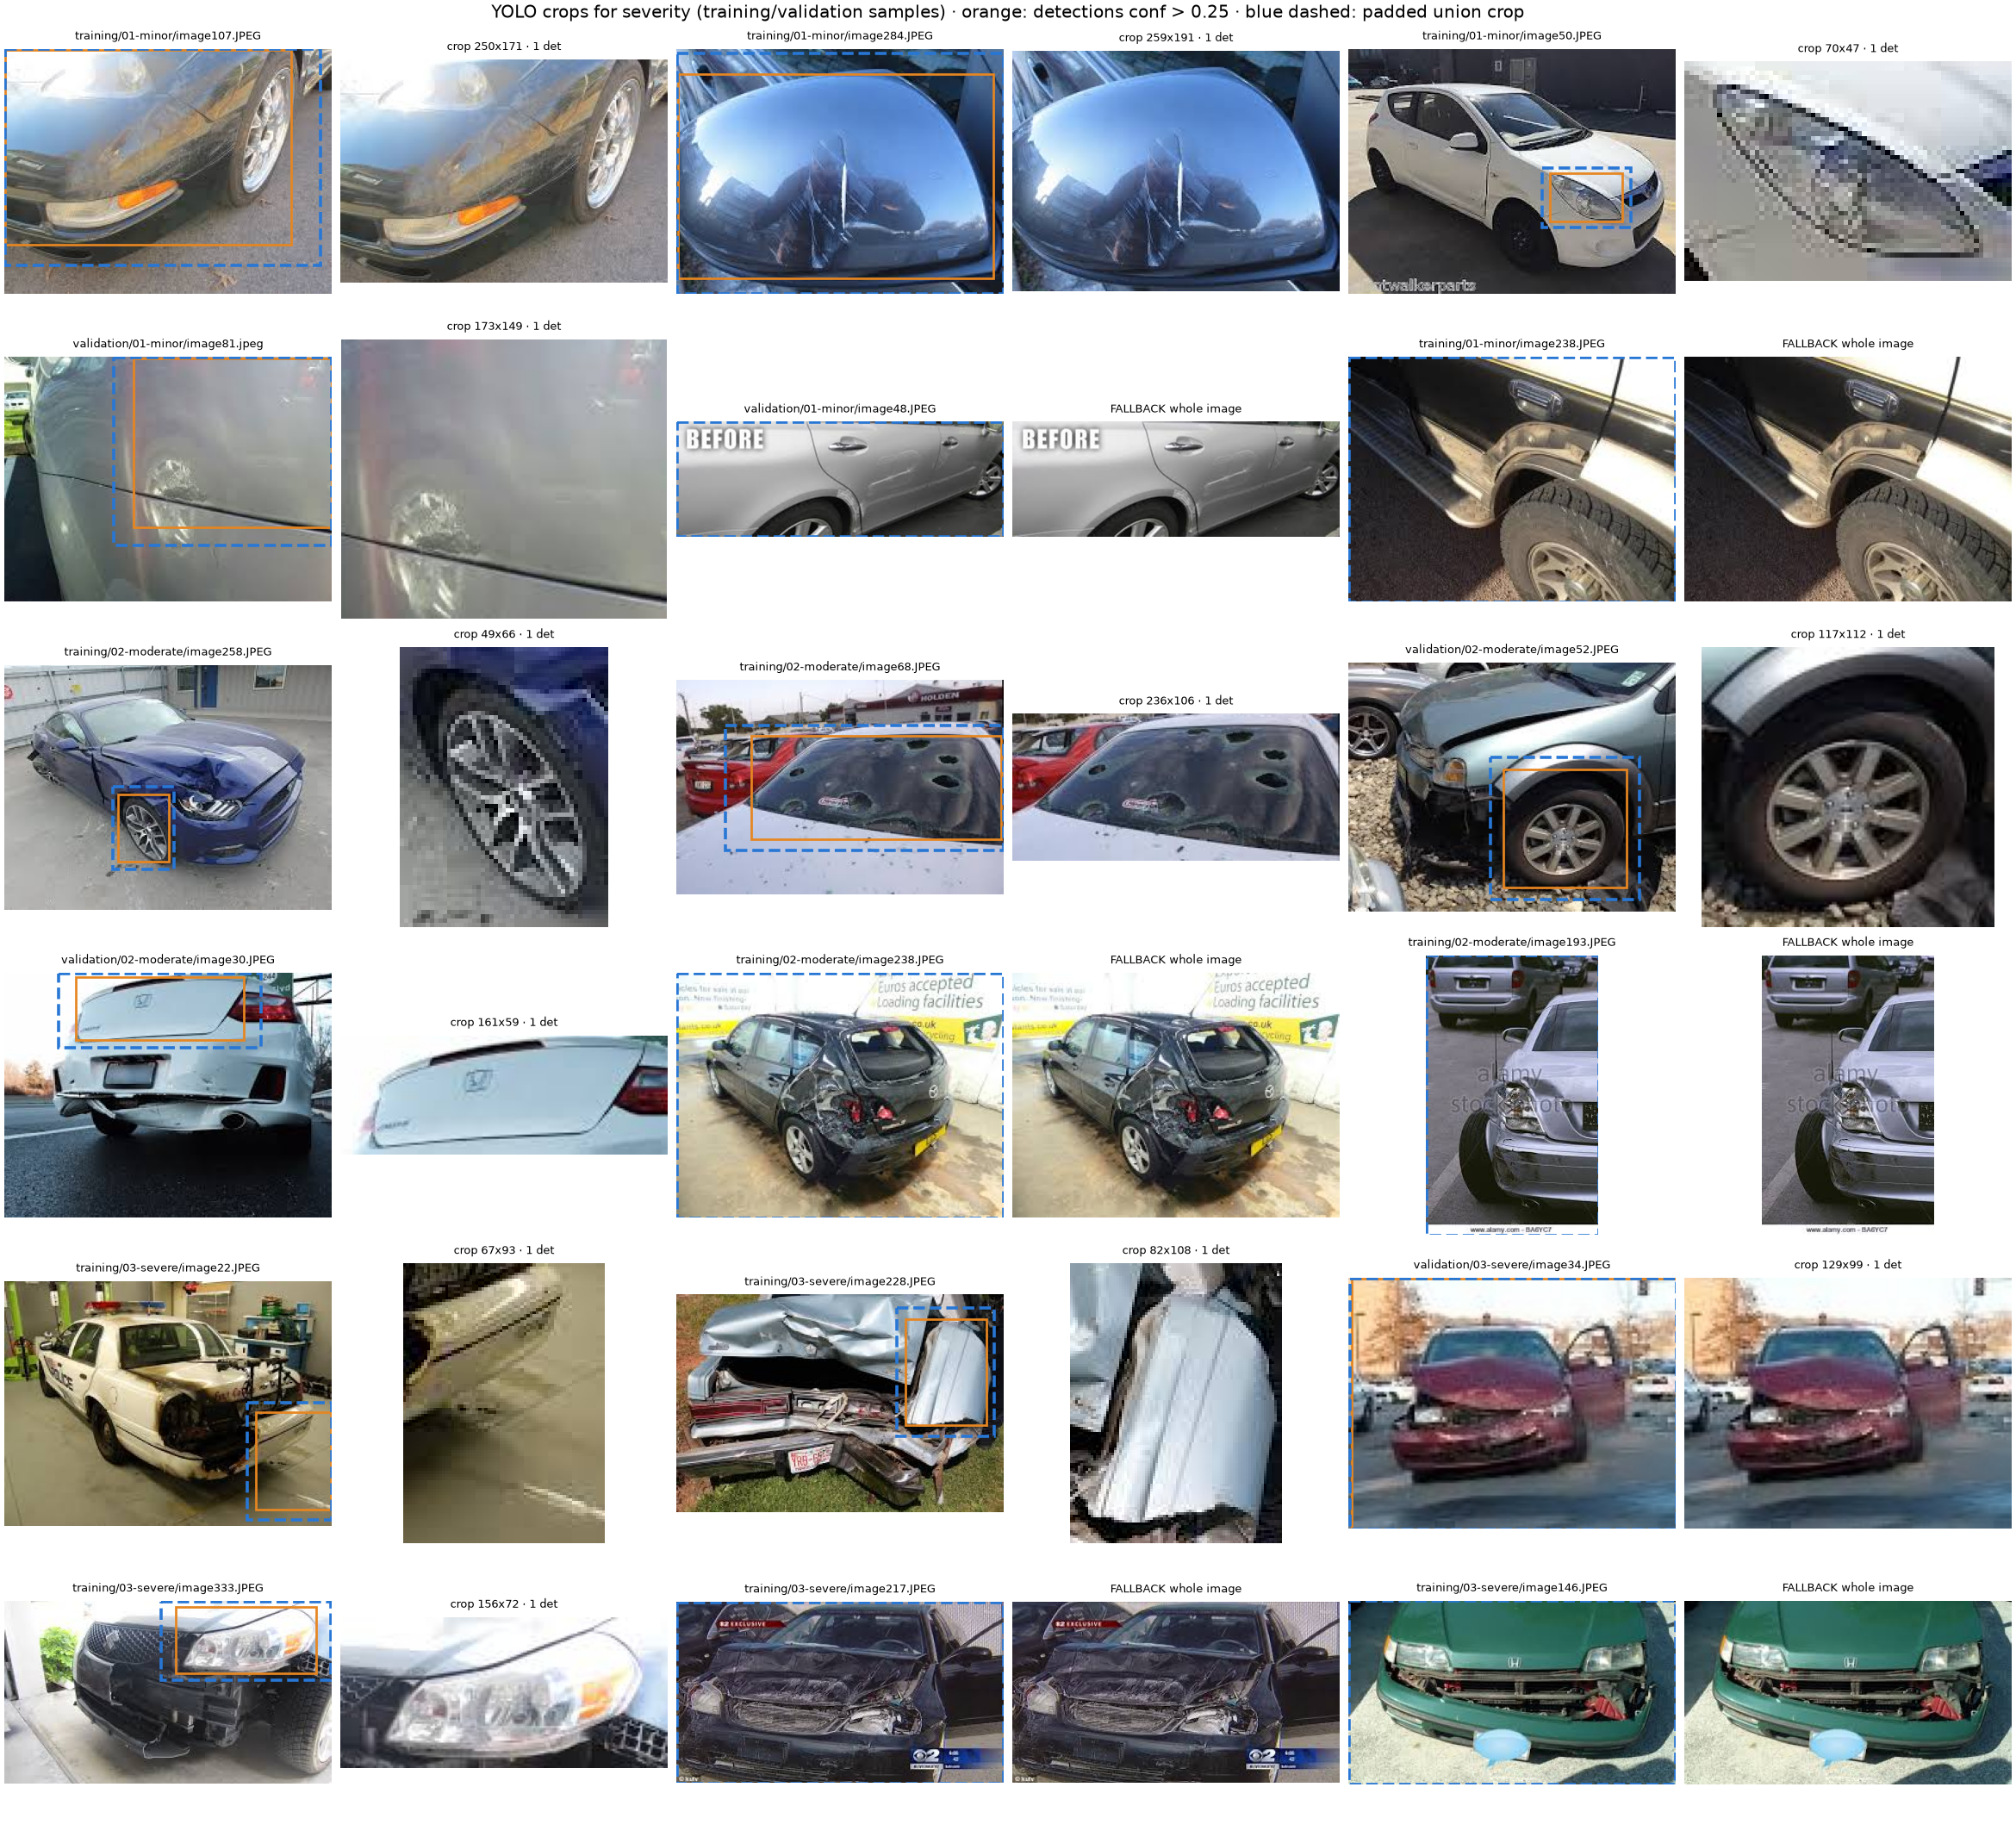
\includegraphics[width=\textwidth]{crop_samples.png}
\caption{Training and validation severity images with YOLO detections (orange) and the resulting padded crop (blue dashed). ``Fallback'' marks images with no detection.}
\label{fig:crops}
\end{figure}

\begin{figure}[!htbp]
\centering
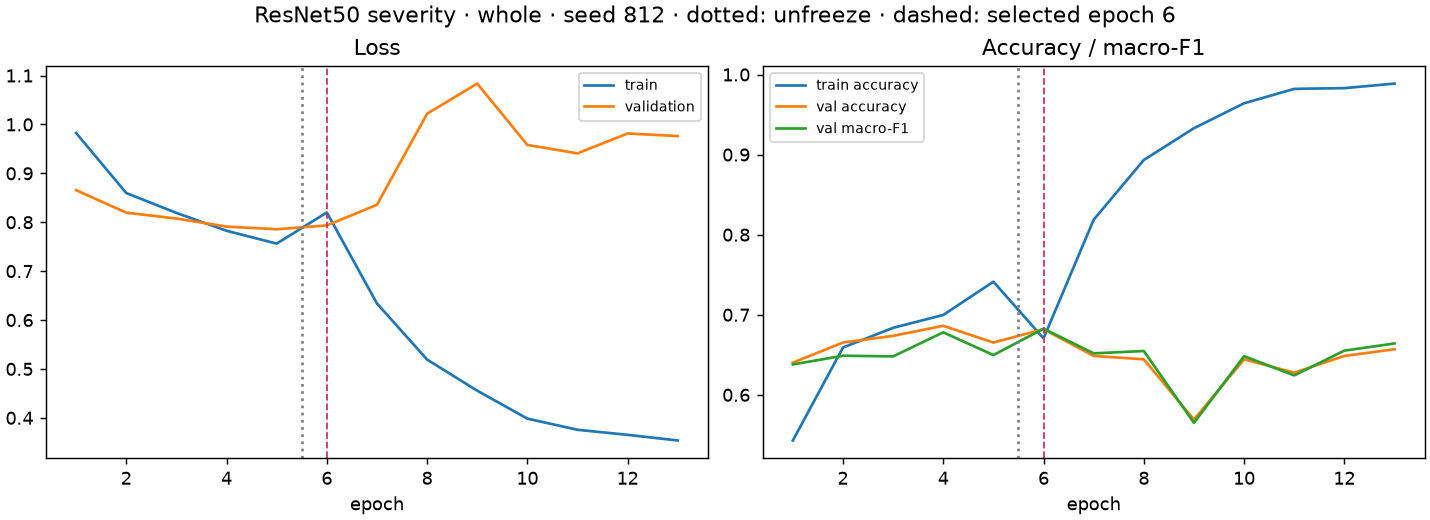
\includegraphics[width=0.85\textwidth]{curves_whole_seed812.png}\\[4pt]
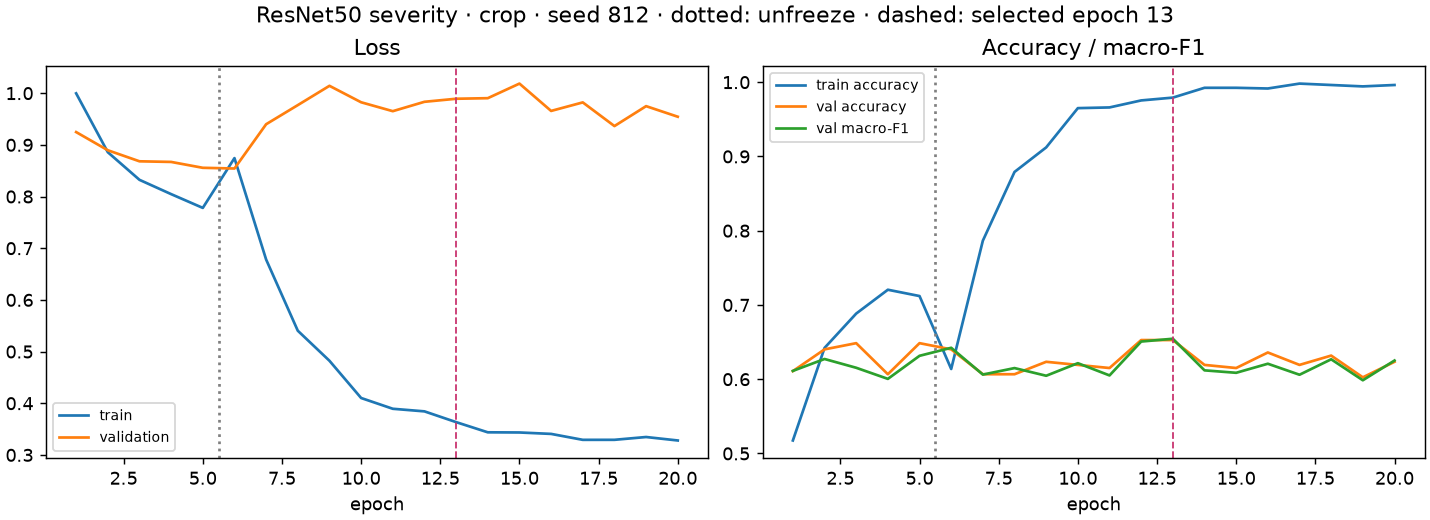
\includegraphics[width=0.85\textwidth]{curves_crop_seed812.png}
\caption{Training curves for seed 812. Top: whole-image system. Bottom: localized system. Dotted line: backbone unfrozen; dashed line: selected epoch. Training accuracy approaches 99\% while validation loss rises, showing overfitting.}
\label{fig:curves}
\end{figure}

\subsection{Results}

The whole-image baseline outperformed the localized system on validation and on test (Table~\ref{tab:sev}, Figure~\ref{fig:sevcmp}). Both systems beat the majority-class baseline of 37.6\% test accuracy.

\begin{table}[!htbp]
\centering
\caption{Severity classification results, mean of three seeds. Brackets give 95\% bootstrap intervals.}
\label{tab:sev}
\small
\begin{tabular}{@{}lrrr@{}}
\toprule
Metric & Whole image & Localized & $\Delta$ (localized $-$ whole) \\
\midrule
Validation macro-F1 (239 images) & 0.683 & 0.646 & $-0.037$ \\
Test macro-F1 (245 images) & \textbf{0.583} [0.533, 0.631] & 0.514 [0.465, 0.562] & $\mathbf{-0.069}$ [$-0.121$, $-0.016$] \\
Test accuracy & 57.7\% & 51.0\% & $-6.7$ points \\
Test recall, minor & 0.806 & 0.662 & $-0.144$ \\
Test recall, moderate & 0.426 & 0.326 & $\mathbf{-0.100}$ \\
Test recall, severe & 0.551 & 0.572 & $+0.021$ \\
Test ordinal MAE (0--2) & 0.448 & 0.531 & $+0.083$ \\
\bottomrule
\end{tabular}
\end{table}

\begin{figure}[!htbp]
\centering
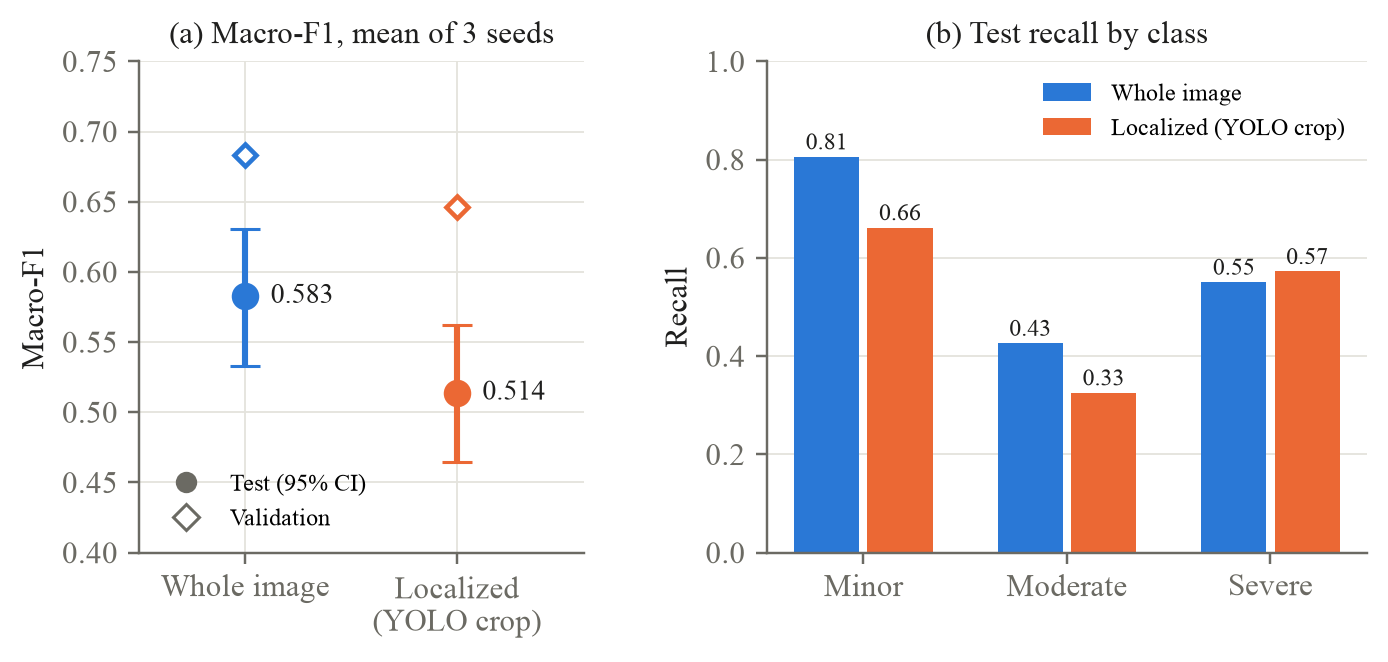
\includegraphics[width=\textwidth]{severity_comparison.png}
\caption{(a) Test macro-F1 with 95\% bootstrap intervals and validation macro-F1. (b) Test recall by class.}
\label{fig:sevcmp}
\end{figure}

To separate the effect of training input from inference input, every classifier was also evaluated on the other input type (Table~\ref{tab:cross}). Cropping at inference costs about 0.05--0.06 macro-F1 for either classifier, and even the crop-trained classifier does better on whole images.

\begin{table}[!htbp]
\centering
\caption{Test macro-F1 by training input and inference input (mean of three seeds).}
\label{tab:cross}
\small
\begin{tabular}{@{}lrr@{}}
\toprule
 & Evaluated on whole image & Evaluated on crop \\
\midrule
Trained on whole image & 0.583 & 0.528 \\
Trained on crop & 0.570 & 0.514 \\
\bottomrule
\end{tabular}
\end{table}

Most errors in both systems are between adjacent severity levels (Figure~\ref{fig:conf}). The whole-image model never classified a minor image as severe. Figure~\ref{fig:err} shows typical errors; several involve images whose label is debatable.

\begin{figure}[!htbp]
\centering
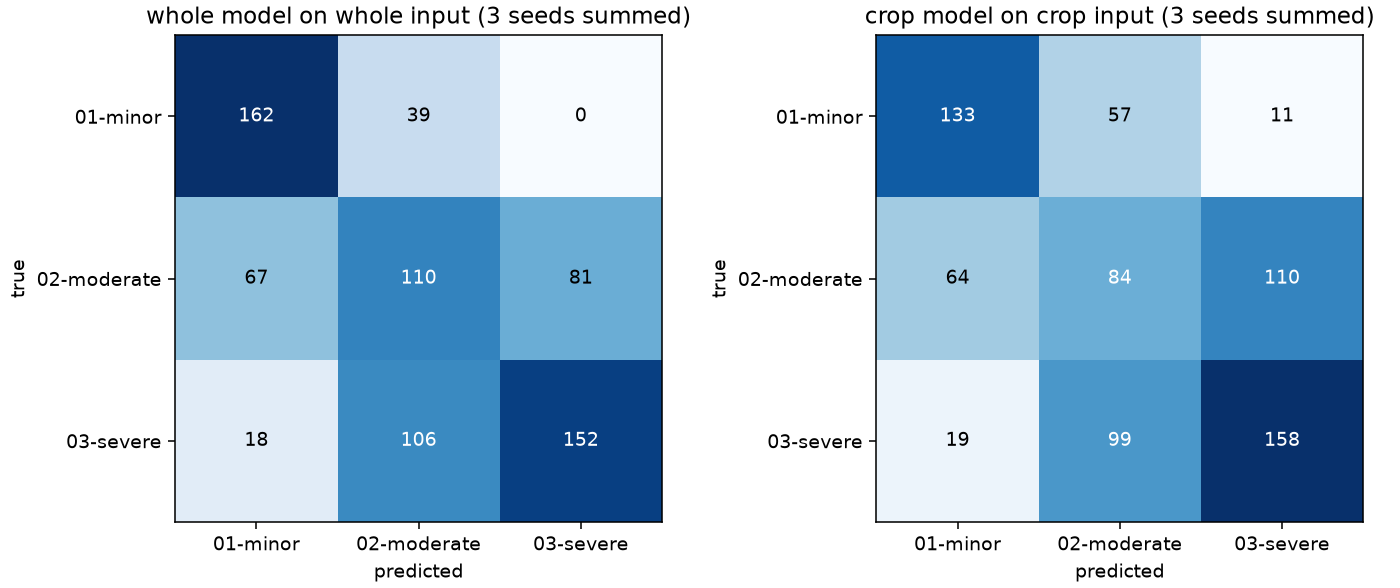
\includegraphics[width=0.92\textwidth]{test_confusion.png}
\caption{Test confusion matrices, summed over three seeds. Left: whole-image system. Right: localized system.}
\label{fig:conf}
\end{figure}

\begin{figure}[!htbp]
\centering
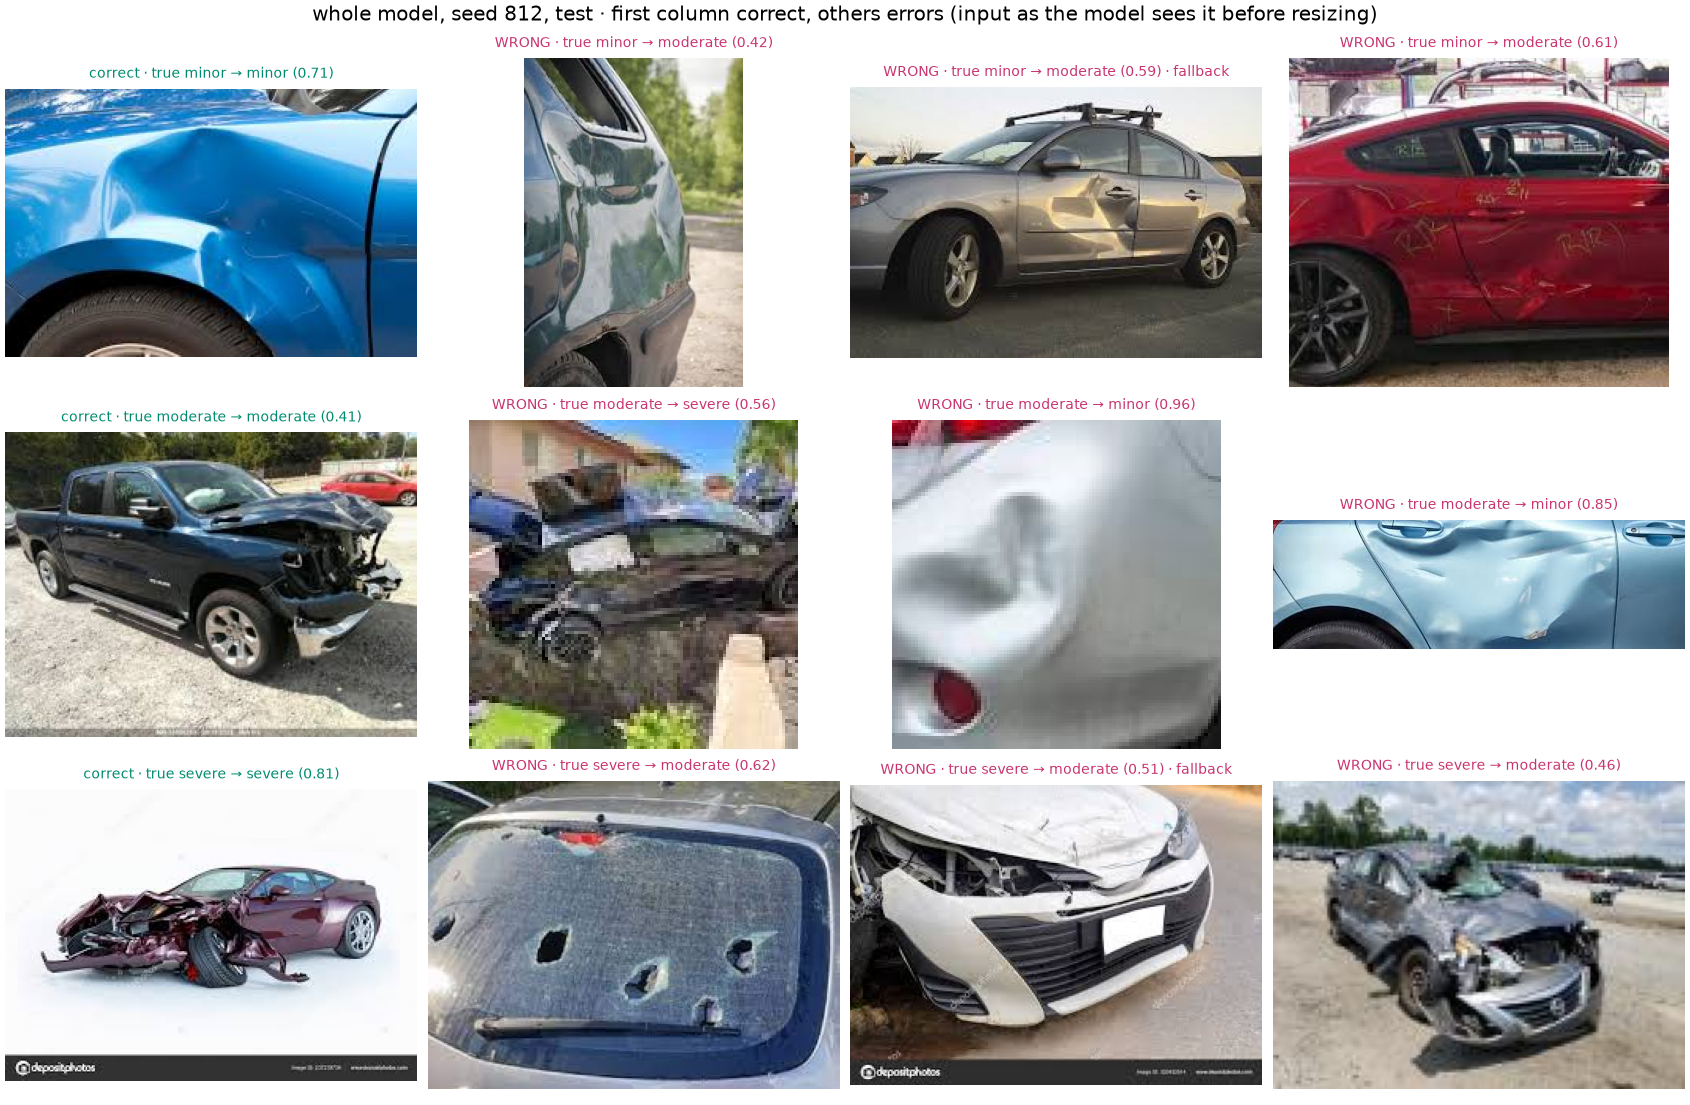
\includegraphics[width=0.92\textwidth]{test_errors_whole.png}
\caption{Whole-image system, seed 812: one correct and three incorrect test predictions per true class.}
\label{fig:err}
\end{figure}

\section{Discussion and Limitations}

The current result answers the research question for \emph{this} detector, not for localization in general. Two explanations given in the proposal are both supported:

\begin{itemize}
  \item \textbf{Detector errors propagate.} The detector misses about half of the severity images and often crops a region away from the main damage.
  \item \textbf{Context matters for severity.} Severity depends on how much of the vehicle is damaged. A tight crop removes that extent, which may explain why minor and moderate recall dropped the most.
\end{itemize}

A domain gap adds to both: the detector learned from CarDD close-ups of dents and scratches, while the severity images are small whole-car photographs, often of heavy crash damage.

Limitations of the current results:
\begin{itemize}
  \item \textbf{Validation is optimistic.} Epochs were selected on validation, and test scores are about 0.10 macro-F1 lower. Test intervals are about $\pm 0.05$.
  \item \textbf{Label noise.} Two image pairs carry conflicting labels, and some labels look questionable on inspection.
  \item \textbf{Fine-tuning added little.} For two of three whole-image seeds, the best epoch came before the backbone was unfrozen.
  \item \textbf{Comparison with earlier projects.} The earlier whole-image model reported 64.7\% accuracy and 24\% moderate recall. Splits and filtering differ here, so the numbers cannot be compared directly.
\end{itemize}

\section{Deviations from the Proposal}

The experimental design follows the proposal. Table~\ref{tab:dev} lists the implementation choices that differ in detail; each is reversible or planned as a variant.

\begin{table}[!htbp]
\centering
\caption{Implementation choices that differ from the proposal.}
\label{tab:dev}
\small
\begin{tabularx}{\textwidth}{@{}p{2.3cm} L L L@{}}
\toprule
Topic & Proposal & Done so far & Remaining work \\
\midrule
Damage regions & One or more boxes, each region classified & One padded union crop per image, since labels are per image & Add per-box classification with an image-level rule \\
No detection & Not specified & Whole image used as fallback & Keep; report with and without fallback images \\
Fine-tuning & Frozen backbone, then selected upper layers & Head only, then all layers & Add upper-layers-only fine-tuning \\
Detector classes & Damage localization & Six damage types merged into one class & Compare with a six-class detector \\
Data filtering & Keep training images out of test & Also removed duplicates, label conflicts and CarDD copies & Keep \\
\bottomrule
\end{tabularx}
\end{table}

\section{Plan for the Remaining Work}

The remaining work asks whether localization helps once the detector is no longer the bottleneck. All tuning uses validation data only.

\begin{enumerate}[label=\textbf{\arabic*.}]
  \item \textbf{Stronger detector.} Retrain YOLO11n for up to 100 epochs with early stopping, train YOLO11s, and train a six-class variant. Choose the model and threshold on CarDD validation, then evaluate the chosen detector once on the CarDD test split.\\
  \emph{Goal:} validation mAP50 and recall clearly above 0.502 and 0.442, with the fallback rate on severity images reported.
  \item \textbf{Localization variants.} On validation only, compare crops from the new detector, crops with 25\% or 50\% padding or a minimum crop size, and per-box classification combined by a fixed rule. Add upper-layers-only fine-tuning for both systems.\\
  \emph{Goal:} one localized and one whole-image configuration, written down before any test run.
  \item \textbf{Final comparison.} Evaluate the recorded configurations once on the 245 test images with three seeds each, and report $\Delta F1$ and $\Delta R_{\text{moderate}}$ with paired bootstrap intervals alongside the first-round result.\\
  \emph{Goal:} both measures reported with intervals, whatever their sign.
  \item \textbf{Moderate-class and error analysis.} Per-class precision, recall and F1; results split by detected and fallback images; Grad-CAM~\cite{gradcam} on the whole-image model to check whether it attends to the damage; visual review of moderate-class errors.\\
  \emph{Goal:} state under which conditions localization helps, as the proposal set out.
  \item \textbf{Literature review.} Related work on damage detection and severity classification~\cite{perez2024,jayaseeli2021,cardd}.
  \item \textbf{Final implementation and demo.} Show whole-image and localized predictions side by side for an uploaded image, using the final models and demo images outside every test split.
  \item \textbf{Final report and oral presentation.}
\end{enumerate}

Figure~\ref{fig:timeline} shows the target schedule. The single fixed point is when the final configurations are recorded, before the one test run. Dates will be aligned with the course deadlines.

\begin{figure}[!htbp]
\centering
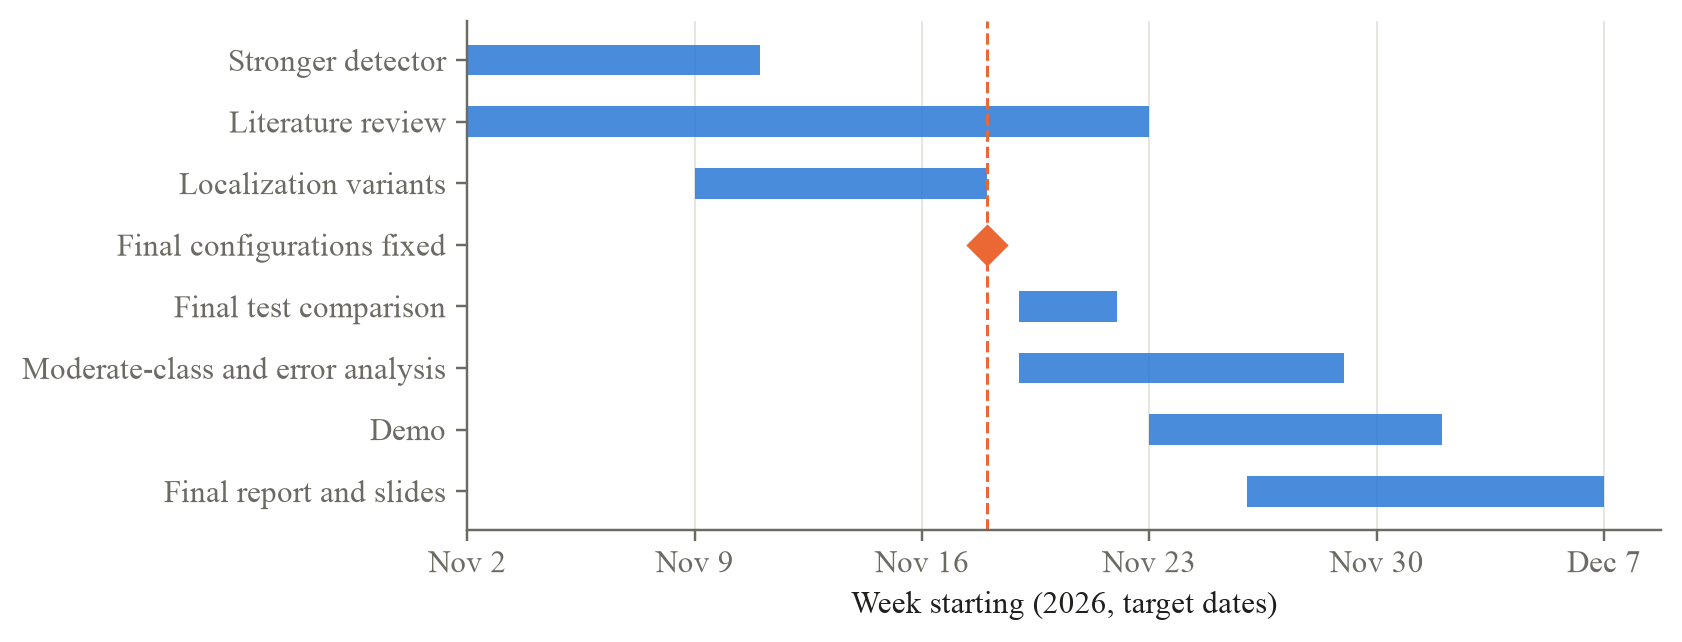
\includegraphics[width=\textwidth]{timeline.png}
\caption{Target schedule for the remaining work. The diamond marks when the final configurations are recorded.}
\label{fig:timeline}
\end{figure}

\section{Risks and Mitigations}

\begin{table}[!htbp]
\centering
\caption{Main risks and how they are handled.}
\label{tab:risk}
\small
\begin{tabularx}{\textwidth}{@{}p{4.2cm} L@{}}
\toprule
Risk & Mitigation \\
\midrule
Second use of the severity test set & Make every choice on validation, record final configurations before the run, evaluate once, report both rounds \\
Better detector still misses most severity-image damage & Report detected and fallback images separately; test crops with more context \\
Small test set (245 images) & Paired bootstrap on the same images; three seeds; report effect sizes \\
Noisy severity labels & Same labels for both systems; document conflicts found in the audit \\
Longer detector training on a laptop GPU & Early stopping; train YOLO11n before YOLO11s \\
\bottomrule
\end{tabularx}
\end{table}

\section{Conclusion}

The project has delivered a working detector, a severity classifier, a controlled comparison and a demonstration dashboard. With the current preliminary detector, whole-image classification outperforms localized classification ($\Delta F1 = -0.069$, $\Delta R_{\text{moderate}} = -0.100$). The remaining work will test whether this holds once detection is no longer the bottleneck, and will explain the moderate-class behaviour, giving the defensible answer that the proposal set as its measure of success.

\begin{thebibliography}{9}
\bibitem{resnet} K. He, X. Zhang, S. Ren, and J. Sun, ``Deep Residual Learning for Image Recognition,'' \emph{Proceedings of the IEEE Conference on Computer Vision and Pattern Recognition (CVPR)}, pp.~770--778, 2016.
\bibitem{gradcam} R. R. Selvaraju, M. Cogswell, A. Das, R. Vedantam, D. Parikh, and D. Batra, ``Grad-CAM: Visual Explanations from Deep Networks via Gradient-Based Localization,'' \emph{Proceedings of the IEEE International Conference on Computer Vision (ICCV)}, pp.~618--626, 2017.
\bibitem{perez2024} S. A. Perez-Zarate, D. Corzo-Garc\'ia, J. L. Pro-Mart\'in, J. A. \'Alvarez-Garc\'ia, M. A. Mart\'inez-del-Amor, and D. Fern\'andez-Cabrera, ``Automated Car Damage Assessment Using Computer Vision: Insurance Company Use Case,'' \emph{Applied Sciences}, vol.~14, no.~20, Art.~no.~9560, 2024.
\bibitem{jayaseeli2021} J. D. D. Jayaseeli, G. K. Jayaraj, M. Kanakarajan, and D. Malathi, ``Car Damage Detection and Cost Evaluation Using Mask R-CNN,'' in \emph{Intelligent Computing and Innovation on Data Science}, Lecture Notes in Networks and Systems, vol.~248, Springer, 2021.
\bibitem{cardd} X. Wang, W. Li, and Z. Wu, ``CarDD: A New Dataset for Vision-Based Car Damage Detection,'' \emph{IEEE Transactions on Intelligent Transportation Systems}, 2023.
\bibitem{yolo11} G. Jocher and J. Qiu, \emph{Ultralytics YOLO11}, software, 2024.
\end{thebibliography}

\end{document}
